\documentclass[11pt]{article}
\usepackage{nsxpreprint}
\usepackage{array}
\AtBeginDocument{\hypersetup{pdfauthor={Ricardo Sandy Aries, SS}}}

\preprintorg{Independent Linguist}
\preprintorginitials{RSA}
\preprintdate{2026-11-01}
\preprintshorttitle{Box by Box: A Japanese-Grounded Revision of Xenogears}
\preprinttitle{Box by Box: Auditing a Xenogears\\Retranslation Against the Japanese}
\preprintauthors{Ricardo Sandy Aries, SS\affil{1,*}}
\preprintlinks{%
  \plink{Base text: Perfect Works Build 0.11.4}{https://github.com/NoharOSP/Perfect_Works_Build}}
\preprintnote{\textsuperscript{*}Corresponding author. Affiliation and correspondence are listed in Appendix~\ref{app:affil}.}

\preprintabstract{%
Fan retranslations of Japanese role-playing games aim to bring a
classic script closer to its original, yet they are usually checked
against whatever source text happens to be public, and the text itself
sits inside compressed binary containers that make every revision a
risk. We report the statistics of \textbf{Box by Box}, a revision audit
of the community Perfect Works retranslation of \emph{Xenogears}, in which
the Japanese original was decoded from the game discs and aligned with
the English script one text box at a time. Revisions were proposed by
SI (Synthesized Intelligence) reviewers under a conservative policy and
were accepted only after a mechanical gate and a reading against the
Japanese line. The audit covered 548,421 Japanese characters and
219,330 English words in 15,987 text boxes across 595 field files,
with 99.7\% of Japanese characters decoded. Of 502 proposals, 492 were
accepted; with six consistency edits this gives 498 revisions, of which
70\% correct meaning errors rather than surface errors. Revisions are
small (median 22 characters) and occur at 2.27 per 1,000 English words,
ranging from 1.07 to 3.04 across the game. A cross-disc comparison
found 376 boxes in 20 disc-2 files that still carried the 1998 script.
The results show that a full source-grounded check of a long game script
is feasible without rebuilding it, and that build consistency is a
translation-quality issue in its own right.}

\begin{document}
\makepreprinttitle

% =====================================================================
\section{Introduction}

Video-game scripts are translated under constraints that most other
texts never meet: fixed text-box sizes, control codes embedded in the
dialogue, and a schedule that ends with the master disc
\citep{ohagan2013game}. Long role-playing games are where these
constraints bite hardest. \emph{Xenogears}, released in Japan in February
1998 and in North America in October 1998 \citep{square1998xenogears},
carries a dense philosophical script whose 1998 English localization was
produced quickly and has been debated ever since.

Fan communities answer such cases with retranslations. The Perfect Works
Build \citep{pwbuild} is a mature example: it ships a revised English
script for both discs of the game, governed by a written style guide and
a list of deliberate name and term choices \citep{pwstyle}. Like any
translation, it benefits from revision by a second linguist working
against the source, the step that service standards make mandatory
\citep{iso17100}. Revision is costly, though, and for a game script it is
costlier still, because the source text is not a document one can open.

Two things make a full revision possible here. First, part of the
Japanese script is publicly transcribed \citep{xgus}, which is enough to
learn how the Japanese disc encodes its characters. Second, the game
stores dialogue as numbered text boxes, so once both discs can be read,
the English and Japanese of each box can be paired by position.

\keypoint{A retranslation checked against a partial source is not
checked.} The public Japanese transcript stops at chapter~6 of a game
with more than sixty, so most of the script had never been compared
with the original line by line.

\keypoint{Fixing the text in isolation does not fix the game.} Each
revision has to survive re-encoding, compression and disc rebuilding
without disturbing the control codes around it, and it has to reach both
discs, which number their files differently.

To address these challenges, we ran a box-by-box audit of the complete
field script and report what it found. We ask four questions: how much
of the script could be aligned with its Japanese source; how many
proposed revisions survived the acceptance gates; what kinds of errors
the revisions correct; and whether the shipped discs agree with each
other. Our contributions are threefold:

\begin{itemize}
\item \contribution{A source-grounded corpus.} We decode the Japanese
discs and align 15,987 text boxes with the English script, covering
548,421 Japanese characters. This turns a partial check into a census.
\item \contribution{Revision statistics.} We report 498 accepted
revisions by category, size and position in the game, together with the
proposals that were rejected and why. The numbers describe where a
mature retranslation still departs from its source.
\item \contribution{A build-consistency finding.} We show that 20 field
files on disc~2 still shipped the 1998 text for scenes revised on
disc~1, and we describe the rule used to repair them. This places build
checks inside translation quality assurance.
\end{itemize}

% =====================================================================
\section{Audit design}

Figure~\ref{fig:pipeline} gives an overview of the audit, from the four
disc images to the rebuilt discs. Each stage either reads data or changes
it under a gate, and nothing reaches the discs without passing every gate
before it.

\begin{figure}[t]
\centering
\begin{tikzpicture}[
  node distance=4mm and 4mm,
  stage/.style={draw=nsxboxline, rounded corners=2pt, fill=nsxlinkbg,
    font=\sffamily\fontsize{7.2}{8.4}\selectfont, align=center,
    minimum height=11mm, text width=23mm, inner sep=2pt},
  gate/.style={stage, fill=nsxaccent!14, draw=nsxaccent},
  data/.style={stage, fill=white, draw=nsxgray},
  arr/.style={-{Stealth[length=2mm]}, draw=nsxink, line width=0.5pt}]
\node[data] (src) {US discs 1--2\\JP discs 1--2\\JP transcript ch.~1--6};
\node[stage, right=of src] (dec) {Decode\\(1,666-code JP\\table)};
\node[stage, right=of dec] (ali) {Align box by box\\(position, padding,\\length)};
\node[stage, right=of ali] (pro) {SI proposals\\(conservative\\policy)};
\node[gate, below=of pro] (g1) {Mechanical gate\\unique, fits box,\\applies to bytes};
\node[gate, left=of g1] (g2) {Reading gate\\against the\\Japanese line};
\node[stage, left=of g2] (wb) {Byte-level\\write-back\\(LZSS, EDC/ECC)};
\node[gate, left=of wb] (ver) {Sector check\\both discs,\\disc-2 sync};
\draw[arr] (src) -- (dec); \draw[arr] (dec) -- (ali); \draw[arr] (ali) -- (pro);
\draw[arr] (pro) -- (g1); \draw[arr] (g1) -- (g2); \draw[arr] (g2) -- (wb); \draw[arr] (wb) -- (ver);
\end{tikzpicture}
\caption{\captiontitle{The audit reads four discs and changes text only
through three gates.} Upper row: data preparation and proposal. Lower
row, right to left: the mechanical gate, the reading gate and the
write-back, followed by verification at sector level on both discs.
Shaded boxes are gates that can reject a change. Schematic; box sizes
carry no meaning.}
\label{fig:pipeline}
\end{figure}

\subsection{Problem formulation}

We treat the audit as a tuple $\mathcal{A} = (B, J, P, G, W)$, where $B$
is the set of English text boxes, $J$ the Japanese boxes paired with
them, $P$ the proposed revisions, $G = (g_1, g_2)$ the mechanical and
reading gates, and $W$ the write-back that turns accepted revisions into
disc sectors. A proposal $p \in P$ names a box $b$, an exact substring
$o$ of $b$, and its replacement $n$. It is accepted when
\begin{equation}
  g_1(p) \wedge g_2(p) = \text{true},
  \label{eq:accept}
\end{equation}
and only accepted proposals enter $W$. Table~\ref{tab:notation} lists
what may change during an audit run.

\begin{table}[t]
\caption{\captiontitle{Only English box text and box size change; every
other object is carried forward unchanged.}}
\label{tab:notation}
\centering\tablefont
\begin{tabular}{@{}lll@{}}
\toprule
\colhead{Object} & \colhead{Change rule} & \colhead{Carried forward} \\
\midrule
Japanese boxes $J$ & read only & yes \\
English box text $b$ & replace substring $o \to n$ & yes, as revised \\
Box size $(w, h)$ & may grow to fit $n$, never shrinks & yes \\
Control codes in $b$ & preserved byte for byte & yes \\
Other file sections & unchanged, except disc-2 sync (\S\ref{sec:sync}) & yes \\
\bottomrule
\end{tabular}
\end{table}

\subsection{Decoding and alignment}

The Japanese disc stores most kana as single bytes and kanji as two-byte
codes. We learned the code table by pairing disc boxes from chapters 1--6
with the public transcript \citep{xgus} and voting on character
assignments, then extended it by inferring the remaining kanji from
context. The final table has 1,666 codes. Main-character names are
stored as name pointers and were expanded to the names they display.

Boxes were paired by position within each field file. Eleven files did
not pair at first. Eight of them turned out to end in empty boxes in the
US build (29 in seven of them), and one Japanese file ends in 29
debug-menu boxes that the US build removed; after these tails were
dropped, the nine files paired one to one. Two files differ by a single box, where the
retranslation splits or repeats a line, and were aligned by a gapped
dynamic program on box length.

\subsection{Proposals and gates}

Reviewers were given the paired boxes, the project style guide
\citep{pwstyle} and a policy: propose a change only for a
mistranslation, an omission of meaningful content, a wrong or missing
speaker, or a clear typo or style-guide violation, and never for tone or
a more literal rendering of a line whose meaning is already right. The
project's deliberate name and term choices were protected.

\parahead{Mechanical gate $g_1$.} A proposal passes when its old text
occurs exactly once in the box, every edited line stays within
28 visible characters (or the page's existing longest line), each page
stays within four lines, and the encoded old text is found exactly once
in the shipped bytes.

\parahead{Reading gate $g_2$.} Each surviving proposal was read against
its Japanese line and accepted, adjusted or rejected. Fixes were copied
to byte-identical boxes in other files only when the text was at least
40 characters long and the edit was not a speaker change; short boxes
such as an ellipsis recur with different speakers.

\subsection{Write-back and cross-disc consistency}
\label{sec:sync}

Revisions replace the encoded substring inside the original box bytes,
so control codes that no text dump exports are kept. The text section is
recompressed, later section offsets are shifted, and a file that
outgrows its sectors is moved to the end of the image. Sector headers,
error-detection and error-correction codes are regenerated. Disc~2 uses
different file indices, so files were matched by content.

A disc-2 file was replaced with its final disc-1 counterpart when three
conditions held: the two files have the same number of boxes and share at
least one box; the Japanese originals of the two files are
byte-identical across the two Japanese discs; and the English text
differs. The first condition rules out lookalike files, and the second
shows that the original game uses one text for both discs.

% =====================================================================
\section{Results}

\subsection{More than half a million Japanese characters were aligned to the English script}

We compared the size of the aligned corpus with the size of the whole
English script, and counted Japanese characters that the code table could
not decode.

The aligned corpus covers 595 field files, 15,987 text boxes,
548,421 Japanese characters and 219,330 English words
(Table~\ref{tab:scope}). This is 86.6\% of the 253,353 English words in
the full script dump, which also contains battle and arena text outside
the field files. Only 1,537 Japanese characters (0.28\%) remained
undecoded. Figure~\ref{fig:scope}a,b splits the corpus by pass: the
first pass, limited to chapters 1--6, accounts for 4.2\% of the aligned
English words.

The ratio of 2.50 Japanese characters per English word is stable across
passes (2.48, 2.50 and 2.53), which suggests that the alignment did not
systematically pair long boxes with short ones.

Three short files, two elevator menus and one Yes/No prompt, have empty
text sections on both Japanese discs; their English was added in the US
build and has no source to check. One further file holds only padding.

\begin{table}[t]
\caption{\captiontitle{The aligned corpus covers most of the script; the
mechanical pass covers all of it.} Counts are full censuses, not
samples. English words exclude control codes.}
\label{tab:scope}
\centering\tablefont
\begin{tabular}{@{}lrrrr@{}}
\toprule
\colhead{Scope} & \colhead{Files} & \colhead{Boxes} & \colhead{JP characters} & \colhead{EN words} \\
\midrule
Pass 1, chapters 1--6 & 18 & 593 & 22,856 & 9,209 \\
Pass 2, chapter 7 to the end & 566 & 15,047 & 509,617 & 203,808 \\
Pass 3, re-aligned files & 11 & 347 & 15,948 & 6,313 \\
\textbf{Japanese-grounded total} & \textbf{595} & \textbf{15,987} & \textbf{548,421} & \textbf{219,330} \\
\midrule
Mechanical pass, whole script dump & 661 & 19,110 & --- & 253,353 \\
Menu strings (disc 1) & --- & 1,950 & --- & 3,879 \\
\bottomrule
\end{tabular}
\end{table}

\begin{figure}[t]
\centering
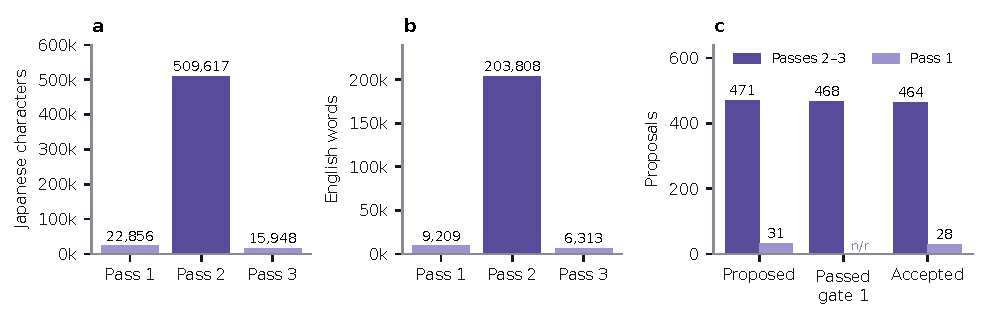
\includegraphics[width=\textwidth]{fig_scope.pdf}
\caption{\captiontitle{Almost every proposal passed the mechanical gate,
and the reading gate removed a further handful.} \textbf{a}, Japanese
characters aligned in each pass. \textbf{b}, English words aligned in
each pass. \textbf{c}, Proposals at each stage. Passes 2--3: 471
proposed, 468 passed the mechanical gate, 464 accepted. Pass 1: 31
proposed and 28 accepted; no separate mechanical-gate count was
recorded (n/r). Measured data.}
\label{fig:scope}
\end{figure}

\subsection{The gates rejected few proposals but caught pipeline faults}

We counted proposals at each stage and recorded every rejection.

Of 502 proposals, 492 were accepted (98.0\%). In passes 2--3, three
proposals failed the mechanical gate (0.6\%) because their old text does
not occur in the shipped bytes, and four more were rejected on reading
(0.9\%). Six revisions did not come from proposals:
five aligned a champion count across files, and one was a copy of an
accepted fix to an identical box in another file. Together these give
498 accepted revisions in 215 of the 595 files (36.1\%).

The gates also caught three faults in the pipeline itself. A first
version of the copy-to-identical-boxes rule spread a one-off speaker fix
to 35 unrelated ellipsis boxes, and copied the fix for a duplicated box
back onto the box that legitimately holds that line; the 40-character
and other-file rules came from this failure. One proposal would have added a speaker name that an earlier
pass had already added. And one box had been reflowed in the script dump but not on the disc,
which the byte-level test detected.

A high acceptance rate is not evidence of high reviewer precision on its
own. The policy asked reviewers to stay conservative, and the reading gate
was applied by the same SI-assisted process that set up the audit, not by
an independent panel.

\subsection{Meaning errors, not surface errors, dominate the revisions}

We classified each accepted Japanese-grounded revision by its error type
and by the reviewer's confidence.

Mistranslations make up 348 of the 498 revisions (69.9\%), followed by
typos (74, 14.9\%), omissions of meaningful content (43, 8.6\%), style
fixes (23, 4.6\%) and speaker fixes (10, 2.0\%), as shown in
Figure~\ref{fig:cat}a. In total, 179 revisions (35.9\%) were marked high
confidence. The separate mechanical pass over the whole script found
surface problems instead: 75 fixes (33 typos, 42 style), 30 text boxes
widened to fit their text, and 18 menu-string rules that changed
69 strings on each disc.

The meaning errors include polarity reversals and lost plot facts.
Table~\ref{tab:examples} shows examples: a farewell that says the
opposite of the Japanese, a radio band named as high frequency where the
Japanese says long wavelength, a box that repeats another box's line
instead of its own, and a dropped clause that explains how a character
escaped.

These categories were assigned by the proposing reviewer and were not
adjudicated against a standard typology such as MQM
\citep{lommel2014mqm}. They map onto its Accuracy branch (mistranslation,
omission) and Fluency branch (typo, style), but the counts are not MQM
scores.

\begin{figure}[t]
\centering
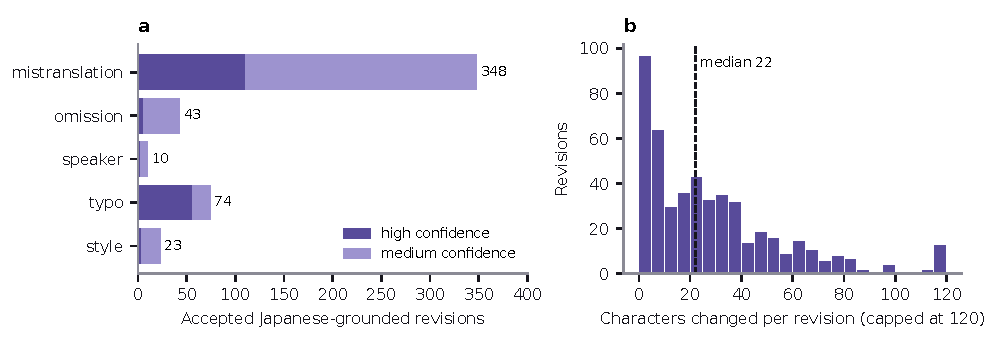
\includegraphics[width=\textwidth]{fig_categories.pdf}
\caption{\captiontitle{Seven in ten revisions correct meaning, and most
revisions change only a few words.} \textbf{a}, Accepted
Japanese-grounded revisions by category, split by reviewer confidence
(n = 498). \textbf{b}, Characters changed per revision, measured as the
total length of non-matching spans between the old and new text, with
tags removed; values above 120 are shown at 120. The dashed line marks
the median. Measured data.}
\label{fig:cat}
\end{figure}

\begin{table}[t]
\caption{\captiontitle{Representative revisions.} Japanese lines are
glossed in English; file and box numbers refer to the field script.}
\label{tab:examples}
\centering\tablefont
\begin{tabular}{@{}>{\raggedright\arraybackslash}p{15mm}>{\raggedright\arraybackslash}p{20mm}>{\raggedright\arraybackslash}p{28mm}>{\raggedright\arraybackslash}p{28mm}>{\raggedright\arraybackslash}p{34mm}@{}}
\toprule
\colhead{Box} & \colhead{Kind} & \colhead{Before} & \colhead{After} & \colhead{Japanese, glossed} \\
\midrule
1640\#5 & mistranslation & It could do with some improvement. & It wasn't half bad. & the brief dream we spoke of was not bad \\
1186\#121 & mistranslation & We can use high frequency \ldots & We can use low frequency \ldots & long-wavelength radio works under water \\
1240\#8 & mistranslation & with Shakhan being so quiet \ldots & Shakhan will not simply stay quiet \ldots & but Shakhan will not keep silent \\
1084\#44 & mistranslation & (copy of box 40) & Something's down here, that's for sure \ldots & it seems certain that something is here \\
1488\#33 & omission & for whose sake he offered to undertake that difficult task & that Nikola risked his life to help escape & the daughter Nikola let escape at the risk of his life \\
1982\#17 & speaker & Hans & Captain & the Captain mocks Hans's cry \\
\bottomrule
\end{tabular}
\end{table}

\subsection{Revisions are small and local}

We measured how much text each revision changed.

The median revision changes 22 characters; 48.2\% change 20 characters or
fewer, and 13.5\% change more than 60 (Figure~\ref{fig:cat}b). Across all
498 revisions the replaced spans grew from 3,769 to 3,887 words (+3.1\%).
Mistranslation and omission fixes have medians of 29 and 30 characters,
against 1.5 for typos and 2 for style fixes.

Small edits matter for a disc game: a revision that fits the existing box
needs no layout change. Only boxes whose new text needs it grow, and no
box shrinks.

\subsection{Error density is uneven along the game}

We grouped files into bands of 150 field-file indices and computed
accepted revisions per 1,000 English words in each band.

The overall density is 2.27 revisions per 1,000 English words, or 9.08
per 10,000 Japanese characters. The density stays between 2.34 and 2.71 in
the first five bands, falls to 1.07 in the band 1650--1799, and rises to
3.04 in the last band (Figure~\ref{fig:density}).

File indices follow the order of the game only approximately, and the
first band mixes pass-1 files with pass-2 files. The bands therefore
describe where revisions concentrate in the script, not a measured
decline in translation quality.

\begin{figure}[t]
\centering
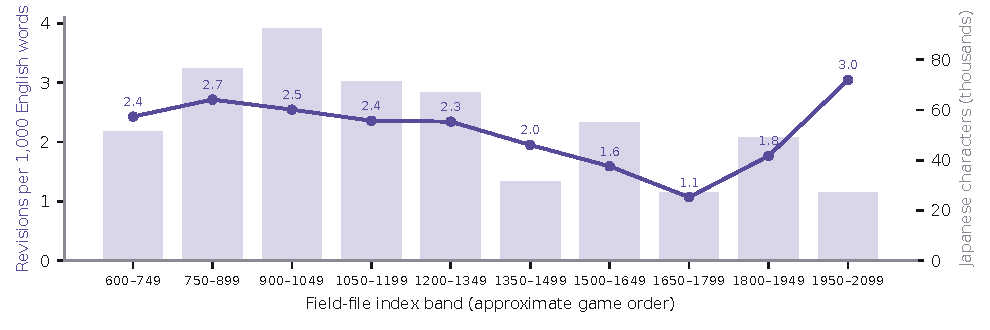
\includegraphics[width=\textwidth]{fig_density.pdf}
\caption{\captiontitle{Revision density varies by a factor of three
across the game.} Line: accepted revisions per 1,000 English words in
each band of 150 field-file indices, with the value labelled. Bars:
Japanese characters aligned in the band, in thousands. Bands are an
approximation of game order. Measured data.}
\label{fig:density}
\end{figure}

\subsection{Build drift left 376 boxes of the 1998 script on disc 2}

Using the rule in \S\ref{sec:sync}, we compared each disc-2 field file
with its disc-1 counterpart and with both Japanese discs.

Twenty disc-2 files met all three conditions. Together they hold
666 boxes, of which 376 (56.5\%) still carried the 1998 localization, for
example ``the Ignas defeat, the Thames retreat'' where disc~1 reads ``the
loss of Ignis \ldots the defeat at the Tamuz'' (Figure~\ref{fig:drift}).
Every Japanese original in these pairs is identical across the two
Japanese discs. Japanese disc~2 holds the disc-1 scenes shifted by nine
file indices and contains no field text that Japanese disc~1 lacks, so
it adds no new source text to the audit.

In five of the twenty files the disc-1 event script also differs from the
original, which is consistent with the gameplay changes the build
describes \citep{pwbuild}. Because the Japanese game uses one script for
both discs, these files were copied whole, but they are the changes most
in need of in-game testing.

\begin{figure}[t]
\centering
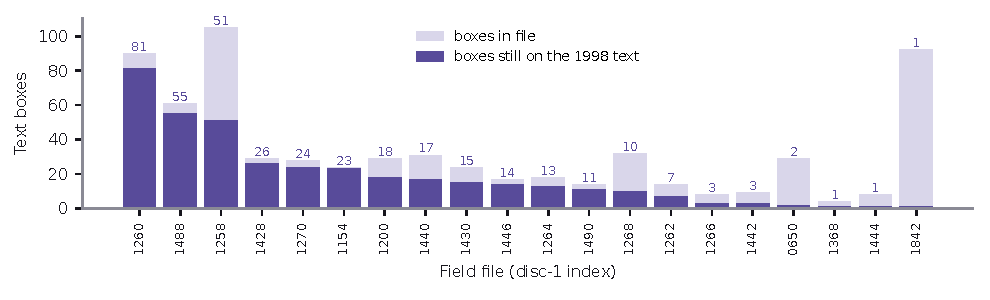
\includegraphics[width=\textwidth]{fig_drift.pdf}
\caption{\captiontitle{Twenty disc-2 files still shipped the 1998 script
for scenes revised on disc 1.} Grey bars: text boxes in the file. Purple
bars and labels: boxes whose English differed from the final disc-1
version. Files are ordered by stale-box count and named by their disc-1
index. Measured data.}
\label{fig:drift}
\end{figure}

% =====================================================================
\section{Related work}

\subsection{Game localization}
Game localization research describes the constraints of box size,
control codes and release schedules that shape a game script
\citep{ohagan2013game}. This work adds a quantitative view of a fan
retranslation, measured against the original text recovered from the
game itself.

\subsection{Translation quality frameworks}
MQM organizes translation issues into a hierarchy with Accuracy and
Fluency branches \citep{lommel2014mqm}, and ISO 17100 requires revision
by a second linguist who compares target and source
\citep{iso17100}. This work applies the revision step to a complete game
script and reports its outcome in categories that map onto MQM's
branches, without claiming MQM scores.

% =====================================================================
\section{Discussion}

The audit shows two things. A complete source-grounded revision of a long
game script is feasible without rebuilding the script: 15,987 boxes were
aligned and 498 revisions were written back as byte-level replacements.
And the remaining errors in a mature retranslation are mostly errors of
meaning rather than of spelling, at a density of about two per thousand
English words.

The idea that made this possible is simple: treat the disc, not a
transcript, as the source of truth for both languages, and let nothing
change the disc unless it applies to the exact bytes that ship. The same
rule exposed the disc-2 drift, which no comparison of script files would
have found.

The audit has limits. No revision has been tested in the running game.
Proposals and acceptance decisions were made by SI-assisted reviewers
under the author's policy, without an independent human panel, so the
category counts and confidence labels carry no measured agreement. The
three US-only boxes, the battle text and the five disc-2 event scripts
remain open, and file-index bands are only a proxy for game order.

% =====================================================================
\section{Methods}

\parahead{Materials.} English text came from the Perfect Works Build
release 0.11.4 \citep{pwbuild}, as both the shipped disc images and the
project's script dump. Japanese text came from images of the two
Japanese discs; disc~2 matched its Redump checksum \citep{redump}. The
public transcript \citep{xgus} was used only to learn the code table and
to pair chapters 1--6.

\parahead{Counting rules.} A Japanese character is any decoded,
non-whitespace character in a paired Japanese box, with name pointers
expanded; control codes and undecoded characters are excluded. An
English word is a run of letters or digits, with internal apostrophes or
hyphens, after control tags are removed. Characters changed per revision
is the total length of the non-matching spans returned by a sequence
matcher on the tag-free old and new text.

\parahead{Verification.} After each build, every changed sector was
checked to belong to an edited file or to the file table; no stray
sectors were found on either disc. Error-detection and error-correction
codes were regenerated and checked on sampled sectors with no
mismatches. Each synced disc-2 file was confirmed byte-identical to its
disc-1 counterpart.

\parahead{Statistical reporting.} All counts are censuses of the full
aligned corpus, not samples, so no confidence intervals are given.
Densities are ratios over the corpus or over a band. Categories and
confidence labels are those assigned at proposal time. Each figure is
produced by a script that reads the project's edit lists and alignment
files directly.

\parahead{Use of SI.} SI systems were used to decode and align the
Japanese text, to propose and vet revisions, and to build and verify the
discs. The author defined the revision policy and the acceptance
criteria.

\bibliographystyle{unsrtnat}
\bibliography{refs}

\appendix
\section{Affiliation and correspondence}
\label{app:affil}
\affil{1}\,Independent Linguist.\\
\affil{*}\,Correspondence: Ricardo Sandy Aries, SS.

\end{document}
